%%「論文」,「レター」,「レター(C分冊)」,「技術研究報告」などのテンプレート
%% v3.3 [2020/06/02]
%% 1. 「論文」
\documentclass[technicalreport]{ieicej}
%\documentclass[invited]{ieicej}% 招待論文
%\documentclass[survey]{ieicej}% サーベイ論文
%\documentclass[comment]{ieicej}% 解説論文
%\usepackage[dvips]{graphicx}
%\usepackage[dvipdfmx]{graphicx,xcolor}
\usepackage[fleqn]{amsmath}
\usepackage{newtxtext}% 英数字フォントの設定を変更しないでください
\usepackage[varg]{newtxmath}% % 英数字フォントの設定を変更しないでください
\usepackage{latexsym}
%\usepackage{amssymb}
\usepackage[dvipdfmx]{graphicx}
\bibliographystyle{sieicej}
\graphicspath{ {./img/} }

\setcounter{page}{1}

\field{}
\jtitle{Beyond 5G高周波通信の空間分解能を 向上するための誘電体導波路の研究}
\etitle{Research on Dielectric Waveguides for Enhancing Spatial Resolution in Beyond 5G High Frequency Communications}
\authorlist{%
 \authorentry{三谷怜司}{Reishi Mitani}{utokyo}\MembershipNumber{}
 \authorentry[nakao@nakao-lab.org]{中尾彰宏}{Akihiro Nakao}{utokyo}\MembershipNumber{}
 \authorentry{福田敦史}{Atsushi Fukuda}{docomo}\MembershipNumber{}
 \authorentry{山本大斗}{Hiroto Yamamoto}{docomo}\MembershipNumber{}
 \authorentry{岡崎浩司}{Hiroshi Okazaki}{docomo}\MembershipNumber{}
 \authorentry{鈴木恭宜}{Yasunori Suzuki}{docomo}\MembershipNumber{}
 %\authorentry{和文著者名}{英文著者名}{所属ラベル}\MembershipNumber{}
 %\authorentry[メールアドレス]{和文著者名}{英文著者名}{所属ラベル}\MembershipNumber{}
 %\authorentry{和文著者名}{英文著者名}{所属ラベル}[現在の所属ラベル]\MembershipNumber{}
}
\affiliate[utokyo]{東京大学 〒113-0033 東京都文京区本郷 7-3-1}{The University of Tokyo, Graduate School of Interdisciplinary Information Studies 7-3-1, Hongo, Bunkyo-ku, Tokyo, 113-0033 Japan}
\affiliate[docomo]{株式会社NTTドコモ 〒239-8536 神奈川県横須賀市光の丘 3-6}{〒239-8536 神奈川県横須賀市光の丘 3-6, 3-6, Hikarinooka, Yokosuka, Kanagawa, 239-8536, Japan}
%\affiliate[所属ラベル]{和文所属}{英文所属}
%\paffiliate[]{}
%\paffiliate[現在の所属ラベル]{和文所属}
\jalcdoi{???????????}% ← このままにしておいてください

\begin{document}
\begin{abstract}
  5G・Beyond5Gで普及が期待されているミリ波などの高周波数帯の通信では
  帯域を広く利用することで大容量の通信が可能となる一方、
  電波伝播の直進性や急激な減衰性から活用の困難さが指摘されている。
  我々は、ミリ波などの高周波数帯の直進性や減衰性を逆に利用し、
  高空間分解能の通信に活用することを考えている。
  アレイアンテナを利用するビームフォーミングでは電波伝播の範囲を
  限定することが可能であるが、一般にコストが高くなるなどの課題がある。
  本研究では、低コストでビームを絞るための誘電体導波路を用いたミリ波アンテナを提案し、
  シミュレーション評価によりその有用性を示す。
\end{abstract}
\begin{keyword}
%和文キーワード 4〜5語
Beyond5G, 誘電体導波路, ミリ波, アンテナ
\end{keyword}
\begin{eabstract}
%英文アブストラクト 100 words
High-frequency communications,
which are used in 5G and expected to be Beyond5G,
enable high-capacity communications by using a wide bandwidth.
However, the high straightness of radio wave
and rapid attenuation
have made it difficult to utilize high-frequency communications.
In this paper, we consider the use of millimeter waves and
other high-frequency communications for high-spatial-resolution communications
by taking advantage of their linearity and attenuation.
Generally, it is possible to limit the range of radio propagation by
beamforming using array antennas in millimeter-wave communications,
but there is a problem of high cost.
In this study,
we propose to design and fabricate a millimeter-wave antenna using
dielectric waveguides to narrow the beam at low cost,
and demonstrate its usefulness through simulation evaluation.
\end{eabstract}
\begin{ekeyword}
%英文キーワード
Beyond5G, Dielectric waveguide, mmWave, Antenna
\end{ekeyword}
\maketitle

\section{はじめに}

第5世代移動通信システム(5G)の商用サービスが2020年3月に開始され、
移動通信システムとしては初めて、28GHz帯を利用した広帯域高速通信が実用化された。
超高速無線データ通信を実現できる28GHz以上のミリ波の利用は
今後拡大されることが予想される。\cite{docomo_6G_white_paper}。

5G・Beyond5Gで普及が期待されている高周波数の通信では、
帯域を広く利用することで大容量の通信が可能となる一方で
電波伝播のLOS(Line-of-Sight)
環境下での伝搬損失やNon-LOS環境下での
急激な伝搬損失の増大への対策が必須となっている。
これらの対策としてアンテナをアレイ化する高利得アンテナの利用がある。
高利得アンテナは高い指向特性を持っていることから
高い空間分解能を得られる可能性があり、
電波が届く範囲を限定することができる。
この特性はセキュリティ対策に利用することができると考えられる。
また、ミリ波は高分解能があるにもかかわらず、
それを生かしたセキュリティを確立する方法が難しい。
ここでいうセキュリティとは以下を示す。

\begin{itemize}
  \item デバイスが多い環境において、それぞれのデバイスへの電波を割り当てること
  \item 渡すべきでない情報を送る電波を不特定のデバイスで受信させないこと
\end{itemize}

しかし、このようなセキュリティ対策を既存の方法では達成するには以下の課題が存在する。

\begin{enumerate}
  \item コスト
  \item リードタイム
  \item インフラが柔軟でないこと
\end{enumerate}

1点目は、
高周波数の電波は波長が短いため、より精密なエンジニアリングが必要となり、
高周波数帯用機器の開発コストが高いためである。
例えば28GHz帯のミリ波の電波伝搬環境を構築する場合には、
高価なアンテナと無線システムが必要となり、
最も簡単な連続波(Continuous Wave: CW)信号
を送受信するだけでも高額な費用がかかる\cite{zep}。
さらに高指向性を得るために
アレイアンテナシステムを用いたビームフォーミングやビームステアリング技術の適用には、
さらなる膨大な費用がかかる。

2点目は、
ホーンアンテナなどの機器は
精密なエンジニアリングが必要となるため納品までに時間がかかるためである。

最後に3点目は、
ホーンアンテナなどの機器は一度配置してしまうと場所を変えにくいため、
最初からメンテナンスがしやすいエリア設計などに気を付けなければならないためである。

そのような課題に対する関連研究に、例えば、
誘電体導波路(以下、導波路)の応用研究
\cite{bending_antenna} \cite{leaky_wave_antenna_bent_dielectric}
がある。
導波路はそれ自体が高周波数帯用の低損失線路であり、
NLOSの原因となる高周波数帯電波の遮蔽物となるものを回避し、
LOS環境を構築できれば、
アンテナ利得を高めるためのアレイ化などは必要なくなり低コスト化が計れる。
また、誘電体の加工のみでよいため、リードタイムの点でも有利である。
さらに、\cite{bending_antenna}
\cite{leaky_wave_antenna_bent_dielectric} \cite{pinching_antenna}
で示される電波放射場所を任意に選べる特長により柔軟なインフラが構築可能となる。
\cite{bending_antenna}では導波路を屈曲することで漏洩した電波による、
エリアの拡張を実証した。
誘電体導波路を曲げて漏れ出した電波を利用し、
エリアの拡張ができることを実証した。
電波伝搬の可逆性により、屈曲箇所は送受信がともに可能なアンテナとなり、
さらに曲げる箇所を変えることで柔軟な電波エリア化が可能となる。
\cite{leaky_wave_antenna_bent_dielectric} \cite{pinching_antenna}
では導波路に別の誘電体を接触させることで、
漏洩した電波によるエリア拡張を実証した。
このような導波路は、
地下街やトンネルなどの通信エリア化のために利用されている漏洩同軸ケーブル
(LCX: Leaky-Coaxial-Cable)と同類と考えることができる。

本研究では、高周波数帯で低損失な特性を持つ導波路と導波路の先端部を
加工した高指向性アンテナで構成される導波路アンテナにより、
高い空間分解能を達成し、
その性能をセキュリティ対策に活用することを検討している。
そこで、
導波路アンテナの設計、製作、測定を通してアンテナとしての指向特性を明らかにし、
セキュリティ対策への有用性を確認する。

本論文の構成は次の通りである。次章では、本研究
に関連する技術について述べる。
第3章では提案手法、
第4章では行った導波路のシミュレーション、
第5章では導波路アンテナの試作について述べ、
そして最終章にて本論文をまとめる。

\section{関連技術}

ミリ波の伝送媒体には主に以下が利用される。
\begin{itemize}
  \item 導波管
  \item 同軸ケーブル
  \item 誘電体導波路
\end{itemize}

図\ref{fig:metallic_waveguide}に示す
導波管は誘電体または空気の周囲を導体で囲んだ断面形状をもち、
ミリ波を含む高周波数帯の伝送線路として利用される。
一般的に導体金属を用いるので、容易に曲げることができず、重い。
図\ref{fig:sma_cables}に示す
同軸ケーブルは中心導体と外部導体が同心円状に配置された断面形状をもち、
おもにマイクロ波以下の周波数帯の伝送線路として利用される。
高周波数帯での損失は導波管よりも大きいという特徴がある。

図\ref{fig:dielectric_waveguide}に示す導波路は
棒状の誘電体(コア)の周囲を異なる誘電率を有する誘電体(クラッド)で囲んだ構造を持ち、
また、レーダーシステム\cite{4297420}などでの利用実績もある。
高周波数帯での損失は同軸ケーブルよりは低く
導波管と比較し軽くて曲げることができる特徴がある。
なお、本研究で用いる導波路は、
コアを比誘電率 2.1 としたポリテトラフルオロエチレン(PTFE)、
クラッドを比誘電率ほぼ 1.00 の空気としたものを用いる。

\begin{figure}[tb]
  %\capwidth=60mm
  %\ecapwidth=60mm
  \begin{center}
    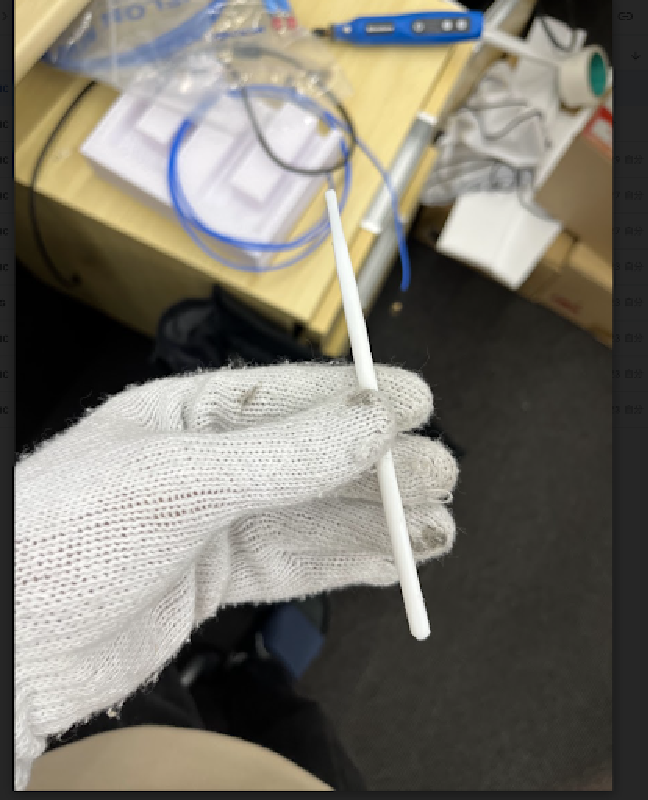
\includegraphics[bb=0 0 311 384, width=0.5\linewidth]{img/waveguide.pdf}
    \caption{誘電体導波路}
    \label{fig:dielectric_waveguide}
  \end{center}
\end{figure}

\begin{figure}[tb]
  %\capwidth=60mm
  %\ecapwidth=60mm
  \begin{center}
    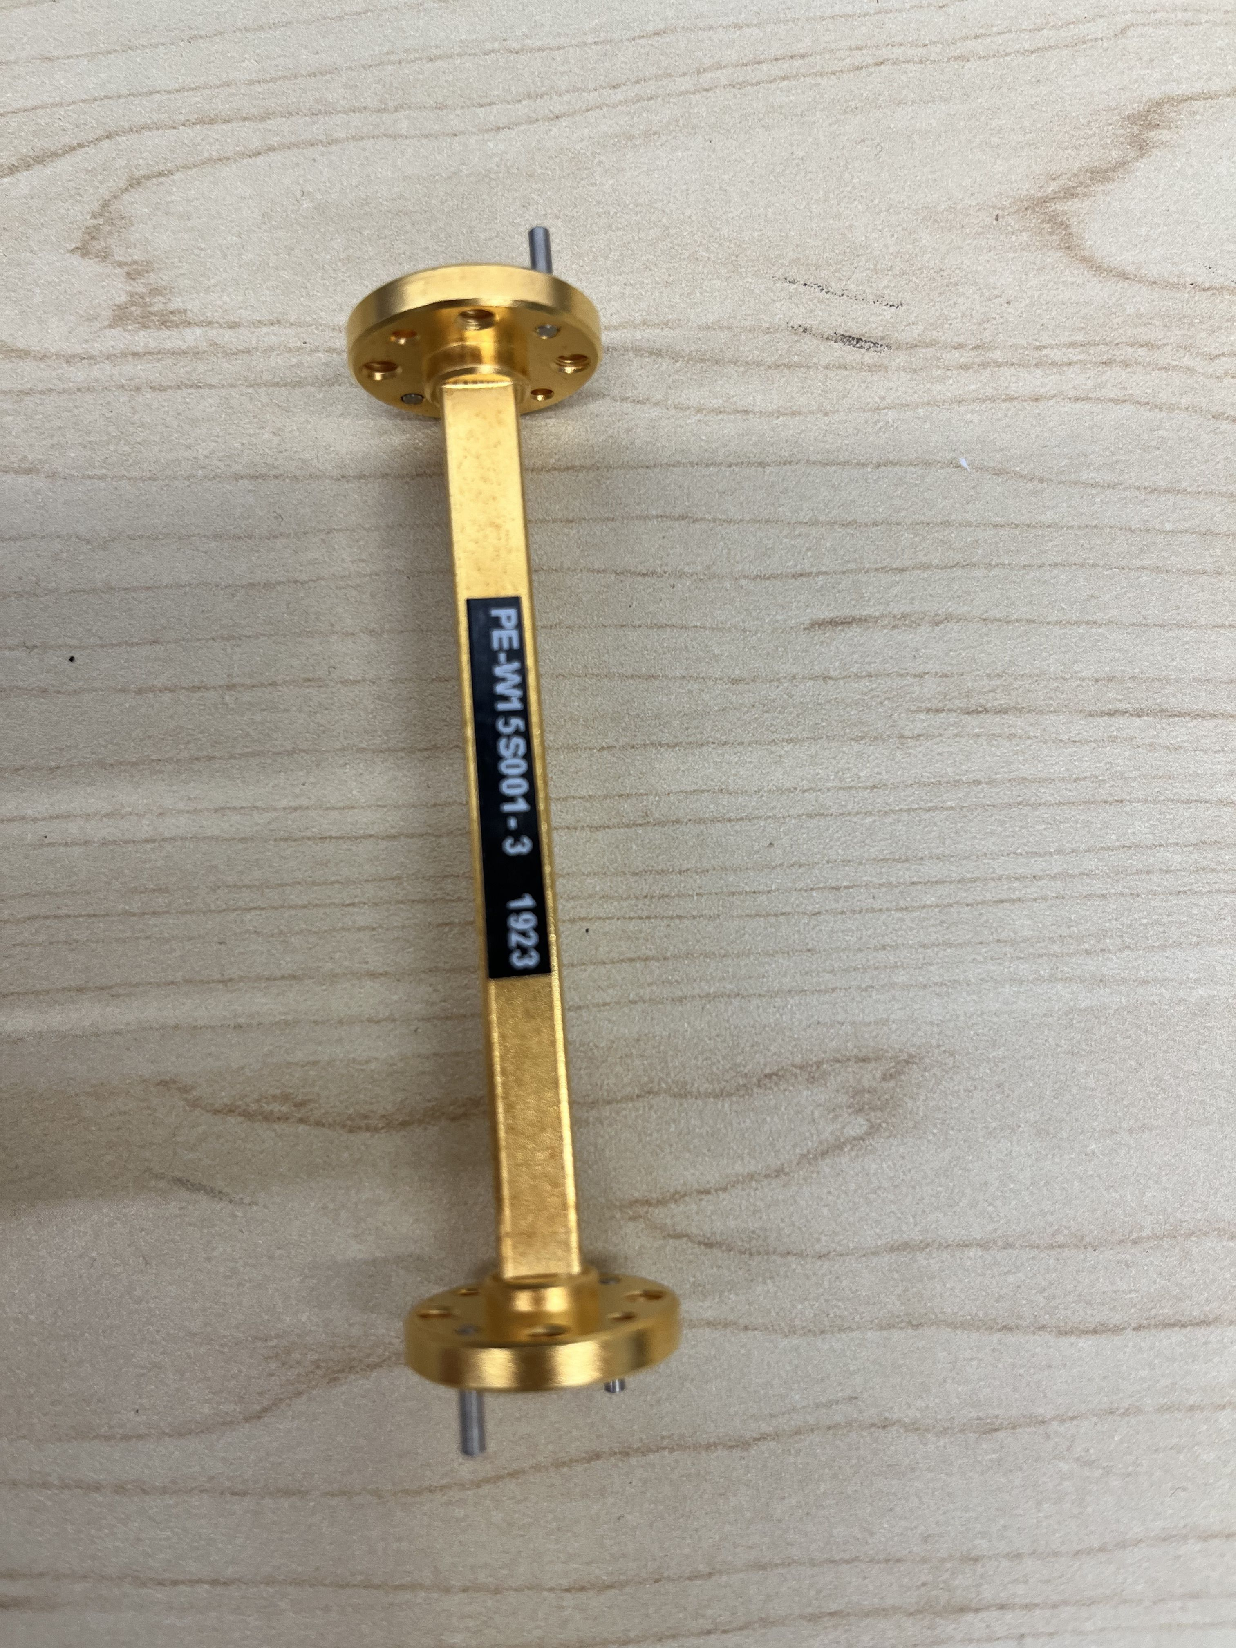
\includegraphics[bb=0.000000 0.000000 593.264305 791.019074, width=0.5\linewidth]{img/metallic_waveguide.pdf}
    \caption{金属導波管}
    \label{fig:metallic_waveguide}
  \end{center}
\end{figure}

\begin{figure}[tb]
  %\capwidth=60mm
  %\ecapwidth=60mm
  \begin{center}
    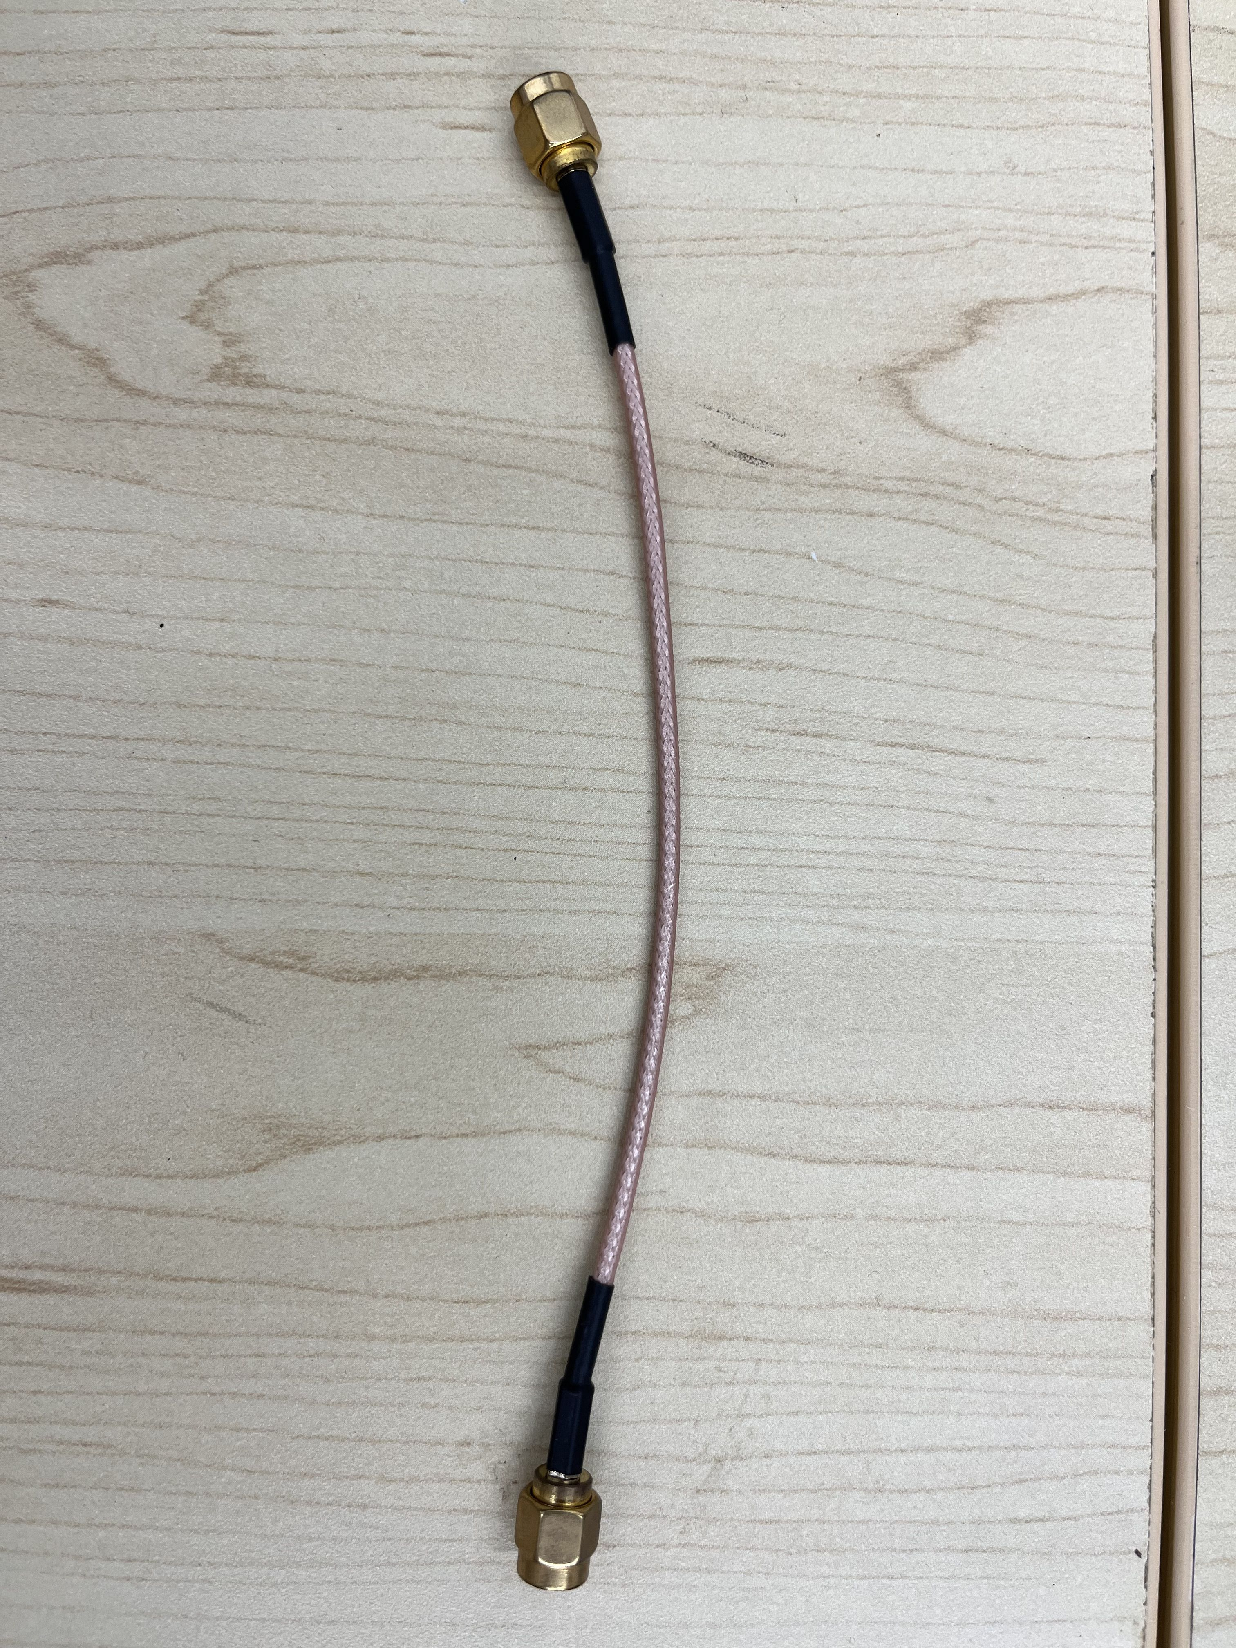
\includegraphics[bb=0.000000 0.000000 593.264305 791.019074, width=0.5\linewidth]{img/sma_cables.pdf}
    \caption{同軸ケーブル}
    \label{fig:sma_cables}
  \end{center}
\end{figure}

\subsection{導波路アンテナ}

本研究では、導波路の先端を加工しアンテナとして機能する導波路アンテナを用いる。
予備実験にて先端を裁断した導波路から電波が放射していることを
確認している。
予備実験ではSHARP社製無線HDMI(High-Definition Multimedia Interface)
送受信ユニット(VR-WH1)を用いた。
主な無線仕様を表\ref{table:wireless}に示す。
本ユニットは。60GHz 帯を使用する Wireless HD 規格の無線送受信ユニットで構成される。
送信機では、入力されたHDMI信号を60GHz帯の広帯域幅(1.76GHz)の電波に変換して出力し、
受信機は受信波からHDMI信号を生成する。

送信機を銅板で囲って電波を遮断した上で
導波路をアンテナ代わりに使う調査実験を行った。
図\ref{fig:qualitative_experiment}
のように導波路アンテナの先端を
受信機に向けているときには動画は再生されるが、
導波路先端が向いている方向を少しでも動かすと動画が再生されないことから、
高い指向特性の放射パターンとなっていることを確認した。

\begin{table}[tb]
  \centering
  \label{table:wireless}
  \caption{無線HDMI送受信ユニットの主な無線仕様}
  \begin{tabular}{lc}
    \hline
    準拠規格 & Wireless HD 1.1 \\
    \hline\hline
    伝送方式 & HTP?LRP \\
    \hline
    中心周波数 & 60.48GHz (Ch2) \\
    \hline
    バンド幅 & 1.76GHz \\
    \hline
  \end{tabular}
 \end{table}

\begin{figure*}[t]
  %\capwidth=60mm
  %\ecapwidth=60mm
  \begin{center}
    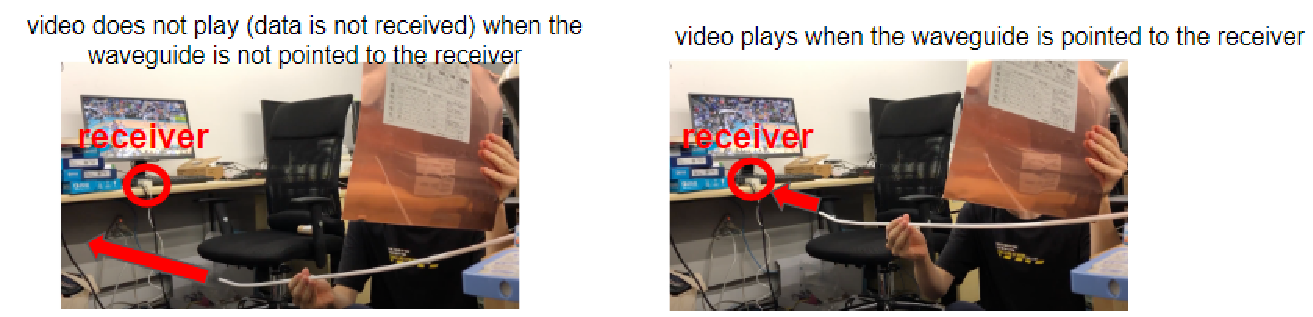
\includegraphics[bb=0 0 630.087950 152.271255, width=1.0\linewidth]{img/qualitative_experiment.pdf}
    \caption{誘電体導波路の予備実験}
    \label{fig:qualitative_experiment}
  \end{center}
\end{figure*}


\section{提案手法}

本研究では導波路アンテナの高い指向特性を利用したセキュリティ対策を提案する。
インターネット社会では個人情報などの秘匿性の高い情報がやり取りされるが、
無線を介する場合には電力解析攻撃によって電波を介した情報漏洩のリスクがある。
例えば、最近は大勢の人がいる ATM の前にて口座情報を確認する、
シェアオフィスにて個人情報を扱う、
など多数の人々・デバイスが存在する環境にて個人情報をやりとりする機会が多くなっており、
そのリスクは上がっている。
高指向性アンテナを用いることで電波の高空間分解能を上げることができるため、
特定の端末のみに電波を放射することが可能となり、
他の端末への情報漏洩を防ぐことができる。
ミリ波の特長である大容量通信を可能にしつつ電波のレイヤーにおいて
秘匿情報を守ることで、セキュリティ対策を行う。
また、導波路アンテナの適用により先に示した問題を解決する。
により端末近傍まで電波を届けることができるため、
アレイアンテナを用いることなく基本的に端末との間にLOS環境を構築できる。
その結果、ハードウェアの開発コストを抑えることができる。
さらに誘電体導波路自体は単純な構造体であり一旦製造工程が確立されれば、
複雑な信号処理を必要とする無線システムを導入するのに比べてリードタイムも縮小できる。
また、導波路は屈曲時の電波漏洩には注意をする必要があるものの、
例えば導波路を室内で引きまわすこともでき、
また軽量であることから、
ホーンアンテナなどの既存の機器に比べてエリアをより柔軟に構築できる。
最後に、高い指向特性を生かして限定したデバイスに情報を渡すことができ、
セキュリティの向上にもつながる。

ここで関連研究と提案手法の比較を行うと
先ほどの誘電体導波路の関連研究は周波数帯利用効率、
設置コスト、設置場所のコスト、そして給電経路の確保において秀でているが、
空間分解能は高くない。
空間分解能を高くしようとすれば、
超多数素子アンテナを用いたアンテナ指向性の制御や分散配置された
基地局アンテナで電波の指向性を制御することができるが
これは逆に設置コスト、設置場所と給電経路の確保が難しくなる。

\subsection{提案手法によって実現できるユースケース}

\begin{figure}[tb]
  %\capwidth=60mm
  %\ecapwidth=60mm
  \vspace{20mm}
  \begin{center}
    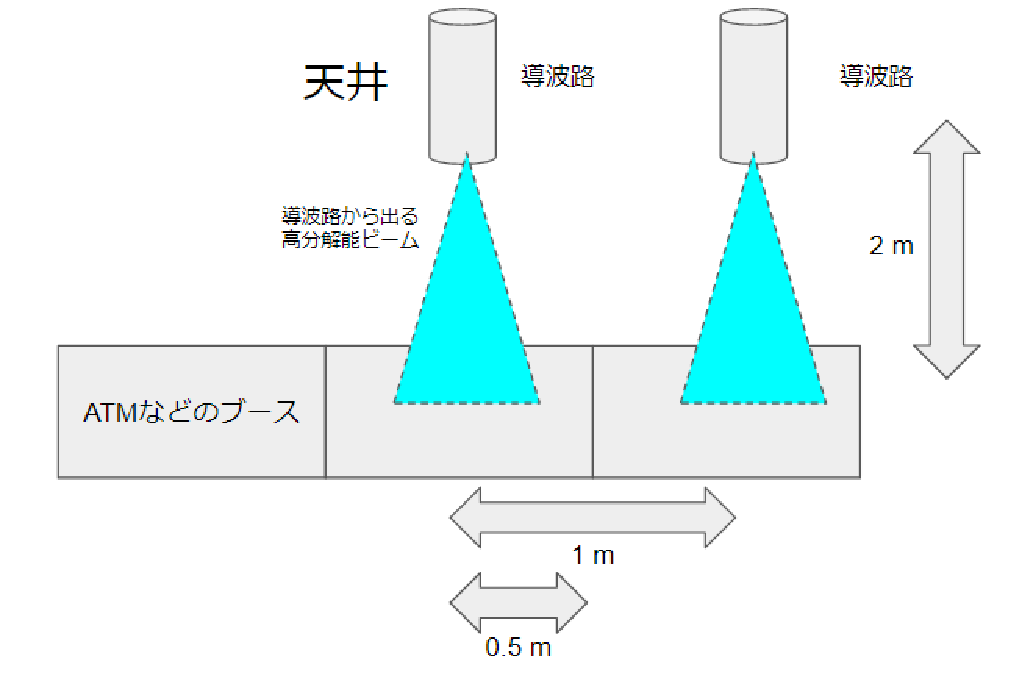
\includegraphics[bb=0 0 384 262, width=0.7\linewidth]{img/usecase.pdf}
    \caption{天井から各ブースへ高分解能ミリ波を提供}
    \label{fig:usecase}
  \end{center}
\end{figure}


例えば図\ref{fig:usecase}のように天井に導波路アンテナを吊るし、
天井から高分解能ビームをユーザー・
デバイスに提供することで物理層におけるセキュアな通信を確立する。
隣のブースへ電波放射しない導波路アンテナの指向特性に対する要求条件は
導波路アンテナまでの高さとブース同士の距離から逆算すればよい。
要求条件は三角関数を使って容易に計算が可能で、
例えば図のように1mおきに狭いブースが並んでいる場合は
$2 * \arctan 0.5 / 2 = 28^{\circ}$の方向にのみ電波を放射する導波路アンテナを設計する。
導波路アンテナの設置場所は、例えば天井裏に導波路を引き廻すことで変更できる。

\section{シミュレーション}

導波路アンテナの指向特性を把握するために 
電磁界シミュレータHFSSを用いて導波路アンテナの3Dモデルをシミュレータ上でモデリングし、
電磁波の指向性を測定計算した。
モデルは導波路先端形状の加工の容易さから
図\ref{fig:normal}に示す先端裁断型、
図\ref{fig:cone}に示すコーン型、
そして図\ref{fig:dome}に示すドーム型の3パターンとした。
導波路の断面は円形とし、先端形状を取り除いた場合の長さは50mm、
直径は10mmである。

\begin{figure}[tb]
  %\capwidth=60mm
  %\ecapwidth=60mm
  \begin{center}
    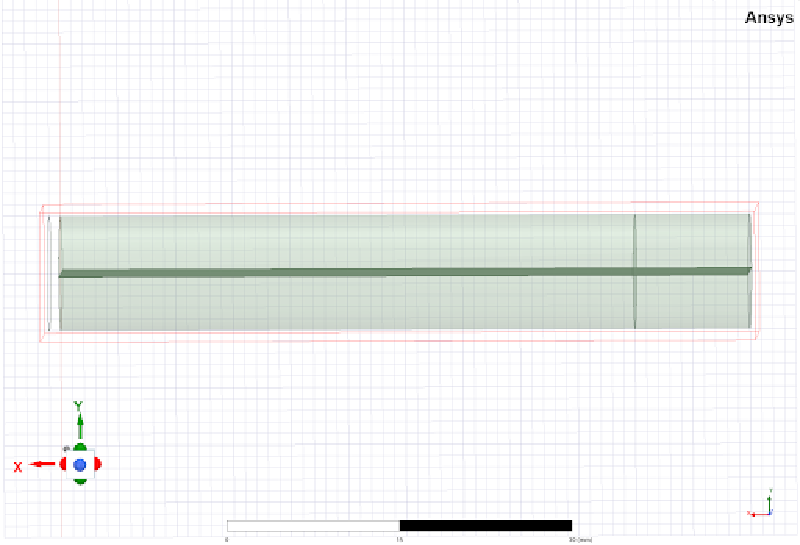
\includegraphics[bb=0 0 384 262, width=0.7\linewidth]{img/normal.pdf}
    \caption{普通の誘電体導波路アンテナ}
    \label{fig:normal}
  \end{center}
\end{figure}

\begin{figure}[tb]
  %\capwidth=60mm
  %\ecapwidth=60mm
  \begin{center}
    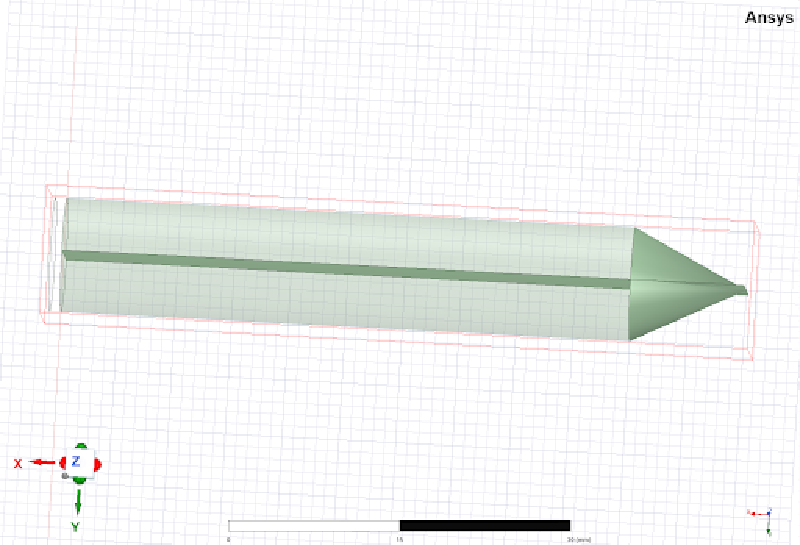
\includegraphics[bb=0 0 384 262, width=0.7\linewidth]{img/cone.pdf}
    \caption{コーン型の誘電体導波路アンテナ}
    \label{fig:cone}
  \end{center}
\end{figure}

\begin{figure}[tb]
  %\capwidth=60mm
  %\ecapwidth=60mm
  \begin{center}
    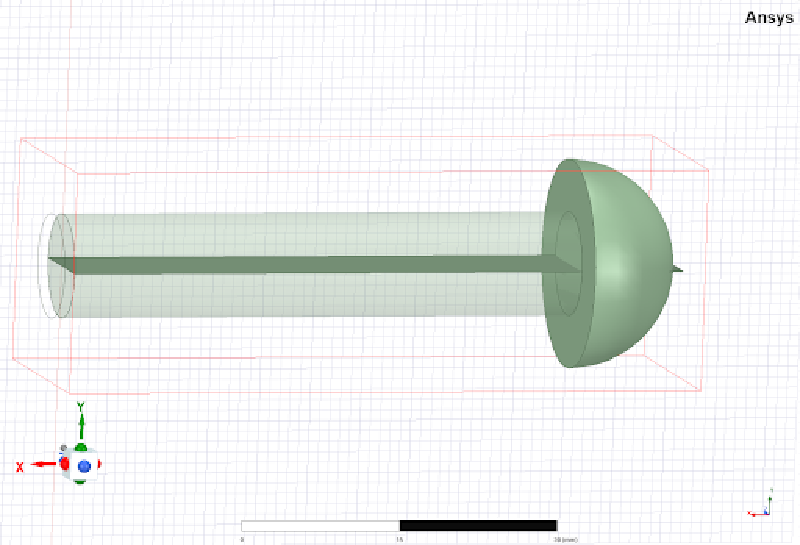
\includegraphics[bb=0 0 384 262, width=0.7\linewidth]{img/dome.pdf}
    \caption{ドーム型の誘電体導波路アンテナ}
    \label{fig:dome}
  \end{center}
\end{figure}

\subsection{シミュレーションの結果と評価}

シミュレーション結果を図\ref{fig:directivity_results}に示す。
50mmで長さを固定した場合については
以下の図\ref{fig:directivity_results}のように
ドーム型が最も高い指向性を示し、ゲインが最大となった。
ドーム型の指向性が図\ref{fig:directivity_results} のように最も高くなった
理由として導波路先端部がその形状からは電波レンズのような効果をもったためと想定される。
コーン型については
形状により外側に電波が広がりやすいため、
他の形状と比較して低い指向特性となったと想定される。

\begin{figure}[tb]
  %\capwidth=60mm
  %\ecapwidth=60mm
  \begin{center}
    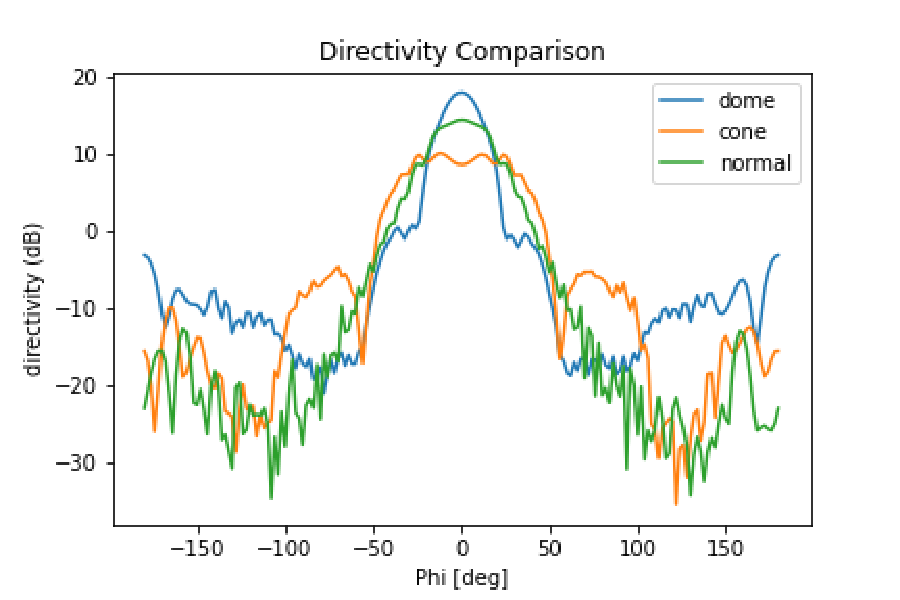
\includegraphics[bb=0.000000 0.000000 432.098422 288.065615, width=1.0\linewidth]{img/directivity_comparison.pdf}
    \caption{指向性の結果}
    \label{fig:directivity_results}
  \end{center}
\end{figure}

\section{導波路アンテナの試作}

最も加工が簡単な先端裁断型の導波路アンテナの試作を行った。
図\ref{fig:docomo_antenna}に製作した導波路アンテナの写真を示す。
また、測定器側のインターフェースとなる同軸ケーブルへ低損失で接続するための
モード変換器も試作した。
まず、試作アンテナへの電波の給電状態を示す反射特性を測定した。
測定結果を図\ref{fig:reflection_params}に示す。
アンテナへの給電を考えた場合、
反射特性として-10 dB以下を目標としており、
該当周波数にて目標を達成していることを確認した。

次に導波路アンテナの
指向性を測定した。
測定は電波暗室内で導波路をその先端を中心として回転させ、
対向側のアンテナで受信した電力を測定した。
図todo, todoに周波数$27GHz$から$29GHz$で$0.5 GHz$刻みの指向特性であり、
図todoは導波路長が20cm、図todoは40cmの結果である。導波路長を変えても、
指向特性に大きな変化は見られなかった。
放射利得が最大利得の半分となる角度範囲を示す半値角はともに36°であった。
したがって、導波路を引き回しても同一先端形状であれば同一指向性が得られ、
実際のユースケースにおいても使用可能と考えられる。
また、先に述べたユースケースで必要とされる半値角の計算値は28°であることから、
目的の指向性に近い値が得られていることが分かった。
図9より先端をドーム型とすることでより高い指向性が得られる可能性がある。

\begin{figure}[tb]
  %\capwidth=60mm
  %\ecapwidth=60mm
  \begin{center}
    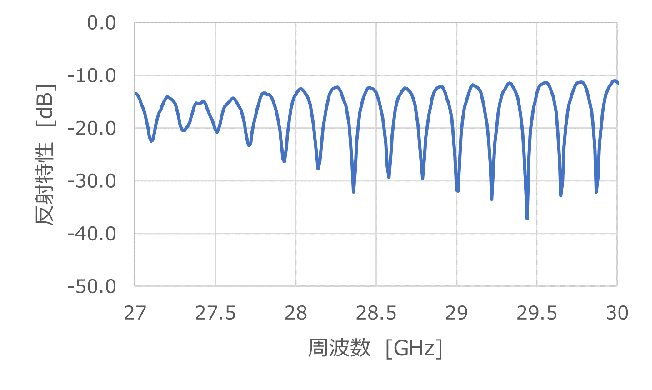
\includegraphics[bb=0 0 408 430, width=0.9\linewidth]{img/reflection_params.pdf}
    \caption{反射特性}
    \label{fig:reflection_params}
  \end{center}
\end{figure}

\begin{figure}[tb]
  %\capwidth=60mm
  %\ecapwidth=60mm
  \begin{center}
    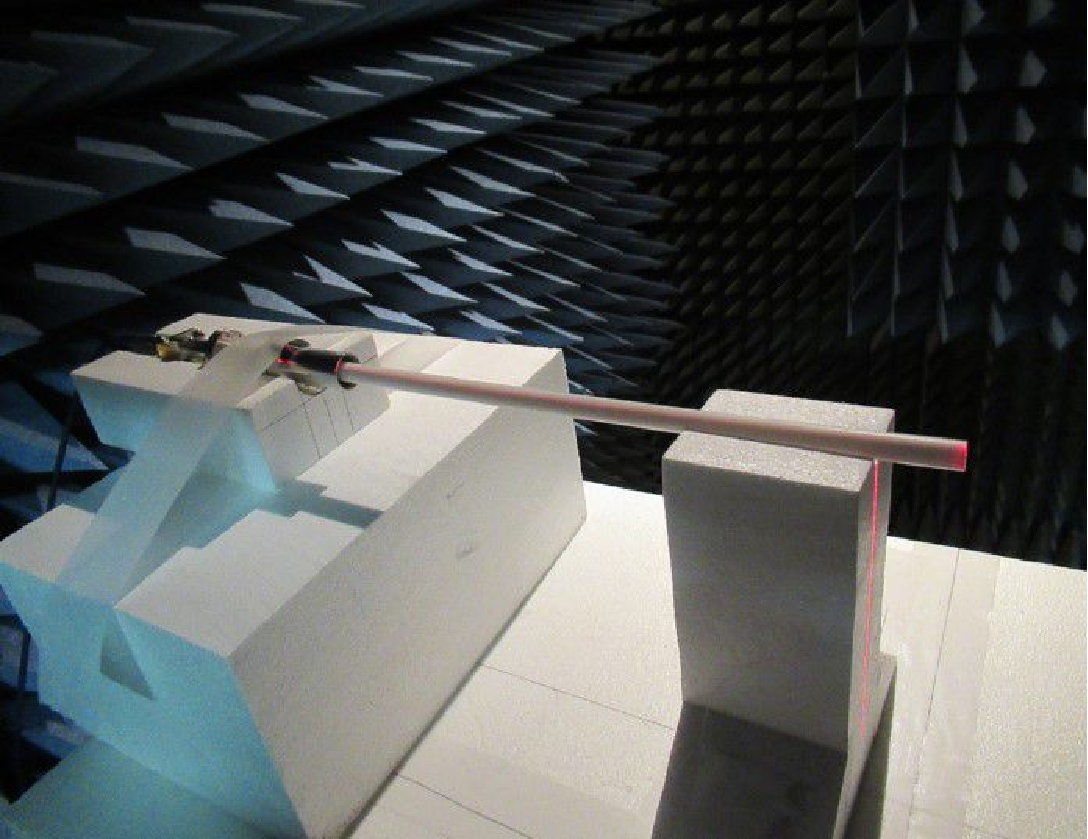
\includegraphics[bb=0 0 408 430, width=0.9\linewidth]{img/docomo_antenna.pdf}
    \caption{試作アンテナ}
    \label{fig:docomo_antenna}
  \end{center}
\end{figure}

\begin{figure}[tb]
  %\capwidth=60mm
  %\ecapwidth=60mm
  \begin{center}
    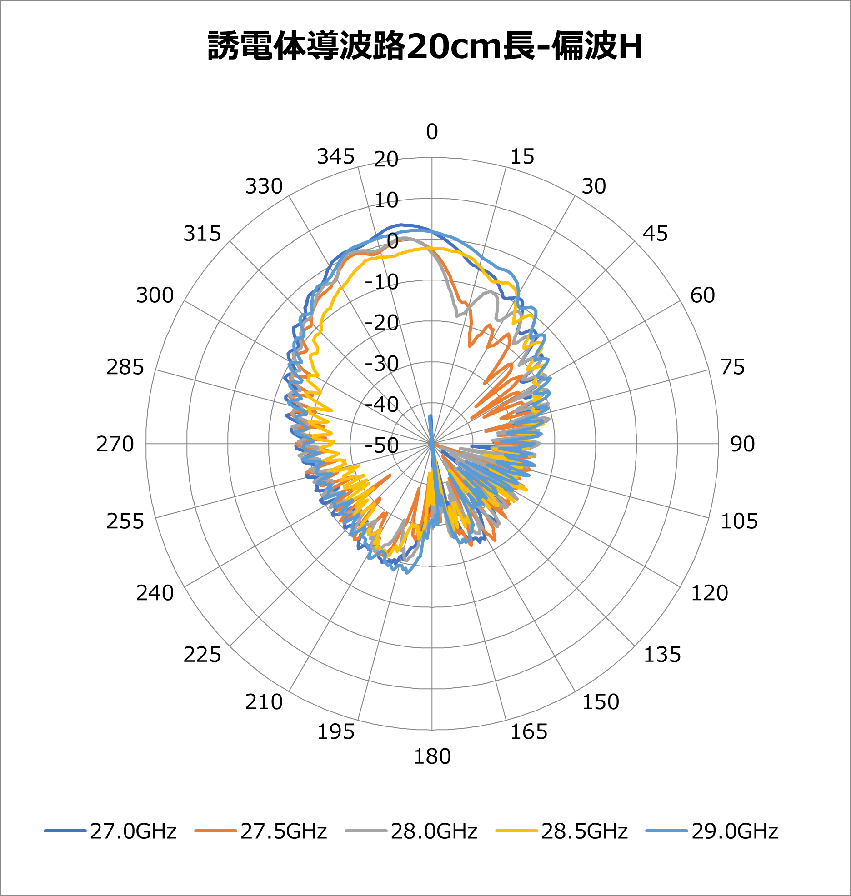
\includegraphics[bb=0 0 408 430, width=0.9\linewidth]{img/waveguide-20cm-h.pdf}
    \caption{20cm長のH偏波}
    \label{fig:20cm-h}
  \end{center}
\end{figure}

\begin{figure}[tb]
  %\capwidth=60mm
  %\ecapwidth=60mm
  \begin{center}
    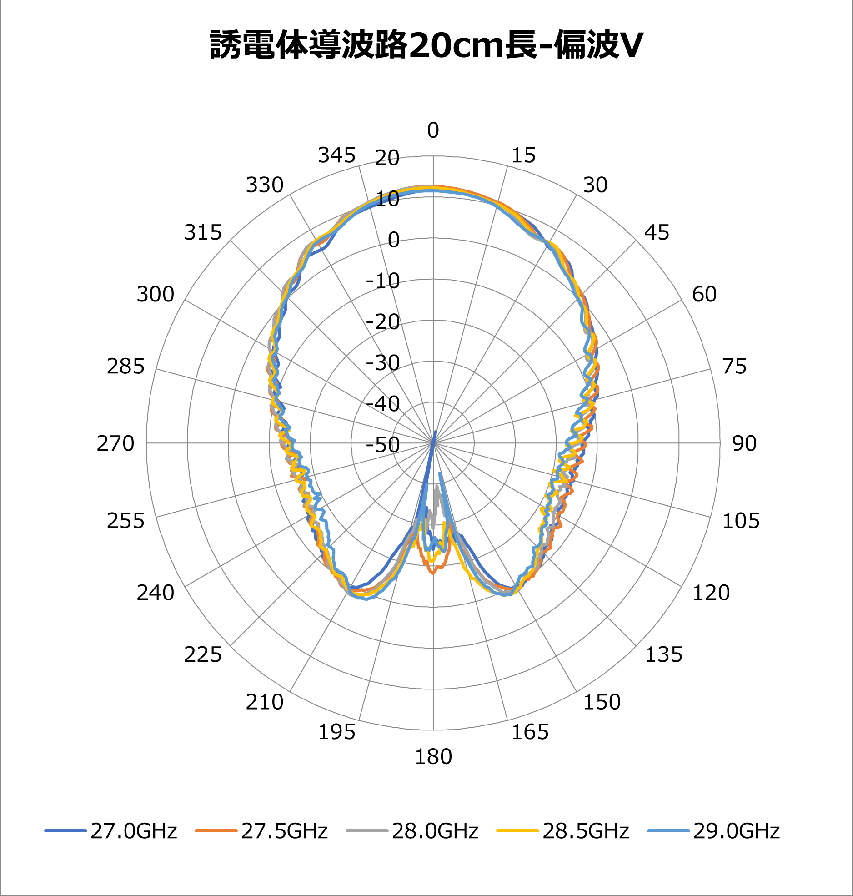
\includegraphics[bb=0 0 408 430, width=0.9\linewidth]{img/waveguide-20cm-v.pdf}
    \caption{20cm長のV偏波}
    \label{fig:20cm-v}
  \end{center}
\end{figure}

\section{今後の展望}

\subsection{異なる形状での利用の検討}

今回はPTFEの導波路に注目して
先端を加工した導波路アンテナの設計および製作を行い、
指向性を確認したが、
PTFEのシートからの電波放射特性の検討を行う予定である。
PTFEシートを用いることで、
一次元のときに比べてユースケースが広がることが期待できる。

\subsection{Local5G環境での使用}

今回の実験は室内または電波暗室の遮断された環境で測定を行ったため、
まだ確認できていない外部要因は多い。
実際にLocal5Gなどの環境では外部要因が多いため、
分解能と減衰率のパフォーマンスの変動があると予想される。
こちらについての考察も今後行っていく。

\section{結論}

本研究では導波路アンテナの高い指向特性を利用したセキュリティ対策を提案した。
高指向性アンテナを有する導波路を設計、製作し、
指向特性を測定した。
測定結果から、
想定されるユースケースで必要とされる条件に近いものが得られることを確認した。
このように、鋭いビームを生かして限定したデバイスに情報を渡すことが可能になれば、
セキュリティの向上につながる。
そしてセキュリティ対策においての課題となる以下を取り払うことができる。

\begin{itemize}
  \item 誘電体導波路を使うことでハードウェアの開発コストやMIMOの開発コストを抑えることが可能となる
  \item 誘電体導波路は短納期が期待でき、リードタイムも縮小できる
  \item 誘電体導波路はある程度曲げても電波の漏れを抑えることができるため、
  誘電体導波路を室内で引きまわしてミリ波の局所エリアを構築することが可能となる。
  また、軽いため、ホーンアンテナなどの既存の機器に比べてエリアをより柔軟に変更できる。
\end{itemize}

\begin{center}
  \Large \textbf{謝辞}
\end{center}

本研究の一部は国立研究開発法人情報通信研究機構 (NICT) 
Beyond 5G研究開発促進事業「Beyond 5Gで実現する同期型CPS
コンピューティング基盤の研究開発」(採択番号: 01201) の助成を受けたものです.

%\bibliographystyle{sieicej}
%\bibliography{myrefs}
\bibliography{common_bibliography}

\end{document}
